% Build from the repository root: make paper
\documentclass[conference,a4paper]{IEEEtran}
\usepackage[T1]{fontenc}
\usepackage{iftex}
\ifPDFTeX
  \usepackage[utf8]{inputenc}
\fi
\usepackage{graphicx}
\usepackage{booktabs}
\usepackage{amsmath}
\usepackage{url}
\urlstyle{same}
% Generated by scripts/build_paper_artifact.py; do not edit.
\newcommand{\AuditCount}{210}
\newcommand{\NpbCount}{120}
\newcommand{\NpbPlainIcGain}{23.84}
\newcommand{\NpbPlainCodeGain}{23.71}
\newcommand{\NpbAttrIcGain}{0.08}
\newcommand{\NpbIcWins}{34}
\newcommand{\NpbIcTies}{37}
\newcommand{\NpbIcLosses}{49}
\newcommand{\NpbAttrCodeGain}{5.76}
\newcommand{\NpbCodeWins}{79}
\newcommand{\NpbCodeTies}{13}
\newcommand{\NpbCodeLosses}{28}
\newcommand{\MibenchCount}{40}
\newcommand{\MibenchPlainIcGain}{1.94}
\newcommand{\MibenchPlainCodeGain}{3.32}
\newcommand{\MibenchAttrIcGain}{-0.70}
\newcommand{\MibenchAttrCodeGain}{1.47}
\newcommand{\BlasCount}{50}
\newcommand{\BlasPlainIcGain}{2.89}
\newcommand{\BlasPlainCodeGain}{0.87}
\newcommand{\BlasAttrIcGain}{2.89}
\newcommand{\BlasAttrCodeGain}{0.95}
\newcommand{\PlainIc}{53,085}
\newcommand{\PlainCode}{291,616}
\newcommand{\PlainBerkeley}{348,878}
\newcommand{\UnrollIc}{40,525}
\newcommand{\UnrollCode}{234,913}
\newcommand{\UnrollBerkeley}{290,559}
\newcommand{\AttrIc}{40,446}
\newcommand{\AttrCode}{214,296}
\newcommand{\AttrBerkeley}{267,814}
\newcommand{\UnrollIcDelta}{12,560}
\newcommand{\AttrIcDelta}{12,639}
\newcommand{\ResidualIc}{79}
\newcommand{\UnrolledModules}{43}
\newcommand{\UnrolledLoops}{449}
\newcommand{\ResidualModules}{5}
\newcommand{\SameIrModules}{114}
\newcommand{\LateCodeDelta}{20,402}
\newcommand{\LateCodeResidual}{215}
\newcommand{\PlainLateCodeDelta}{14,902}
\newcommand{\ExamplePlainIc}{90}
\newcommand{\ExamplePlainBytes}{377}
\newcommand{\ExampleUnrollIc}{25}
\newcommand{\ExampleUnrollBytes}{119}
\newcommand{\ExampleAttrIc}{25}
\newcommand{\ExampleAttrBytes}{87}
\newcommand{\SourceCount}{12}
\newcommand{\SourcePlainBytes}{38,315}
\newcommand{\SourceAttrBytes}{32,410}
\newcommand{\SourceClangBytes}{32,123}
\newcommand{\SourceAttrOverClang}{0.89}
\newcommand{\GsmOverClang}{12.81}
\newcommand{\SelectorCount}{347}
\newcommand{\GnnCodeMin}{2.84}
\newcommand{\GnnCodeMax}{3.66}
\newcommand{\GnnBerkeleyWithoutMin}{1.35}
\newcommand{\GnnBerkeleyWithoutMax}{2.06}
\newcommand{\RandomCodeMin}{2.82}
\newcommand{\RandomCodeMax}{3.68}
\newcommand{\RandomBerkeleyWithoutMin}{-0.28}
\newcommand{\RandomBerkeleyWithoutMax}{1.76}

\newcommand{\PairedRows}{%
NPB (120) & Portfolio & 23.84 & 0.08 & 23.71 & 5.76 \\
NPB (120) & Random & 22.35 & -1.87 & 24.53 & 6.46 \\
MiBench (40) & Portfolio & 1.94 & -0.70 & 3.32 & 1.47 \\
MiBench (40) & Random & 0.62 & -2.06 & 2.39 & 1.00 \\
BLAS (50) & Portfolio & 2.89 & 2.89 & 0.87 & 0.95 \\
BLAS (50) & Random & 2.26 & 2.26 & 0.80 & 1.14 \\
}

\setlength{\textfloatsep}{8pt plus 2pt minus 2pt}
\setlength{\dbltextfloatsep}{8pt plus 2pt minus 2pt}

\begin{document}
\title{A Causal Audit of Baselines for\\LLVM Code-Size Optimization}
\author{\IEEEauthorblockN{Dimitrije Pe\v{s}i\'c}
\IEEEauthorblockA{School of Electrical Engineering, University of Belgrade\\
Belgrade, Serbia\\pd230014d@student.etf.bg.ac.rs}}
\maketitle

\begin{abstract}
A large improvement over a compiler baseline can depend on how the
baseline's input is prepared. We investigate this effect in an LLVM
phase-ordering experiment using the original CompilerGym service.
Adding function size attributes to both reference and candidate inputs
changes a fixed portfolio's instruction-count gain on \NpbCount{} NPB
modules from \NpbPlainIcGain\% to \NpbAttrIcGain\%.
A controlled intervention that prevents loop unrolling removes
\UnrollIcDelta{} of the \AttrIcDelta{} additional instructions in the
original reference. Measurements on fixed optimized IR separately
identify an attribute-dependent code-generation effect. The corrected
comparison still retains \NpbAttrCodeGain\% savings in code-section
bytes, so the instruction-count result does not determine the native
size result. Paired measurements on three suites, a small source-build
control, and a learned-versus-random selection check delimit the finding.
We provide per-module records and an executable example to make baseline
preparation, causal interventions, and size definitions inspectable.
The study concerns the audited protocol and does not establish errors
in other CompilerGym-based results.
\end{abstract}

\begin{IEEEkeywords}
compiler optimization, LLVM, code size, phase ordering, reproducibility
\end{IEEEkeywords}

\section{Introduction}
Choosing a sequence of compiler optimization passes is often evaluated
by comparing the resulting intermediate representation (IR) with a
standard optimization pipeline. CompilerGym~\cite{compilergym} makes
this experiment accessible through a common interface, including an
LLVM \texttt{-Oz} reference and a fast instruction-count objective.
Learned methods can select passes or choose from a portfolio of
sequences~\cite{coreset}. The practical motivation is smaller deployed
code, but two distinctions matter: applying a named pipeline to existing
IR is not necessarily equivalent to compiling source code with that
optimization level, and counting IR instructions is not the same as
measuring the generated machine code.

We encountered both distinctions while evaluating a fixed portfolio
and a learned pass-ordering policy. On \NpbCount{} NPB modules, eight
portfolio candidates appeared to reduce the summed instruction count
by \NpbPlainIcGain\% relative to CompilerGym's \texttt{-Oz} reference.
Giving both sides the function attributes used for size optimization
reduces that advantage to \NpbAttrIcGain\%. Such a change warrants an
explanation before interpreting the original result as an improvement
over compilation for size.

This paper asks: \emph{which part of the apparent improvement is
sensitive to input preparation, and which compiler decisions explain
that sensitivity?} We keep the original LLVM service and candidate
sequences fixed. A paired experiment measures the attribute effect;
an intervention on loop metadata tests unrolling; and attributes added
only after IR optimization isolate their effect during code generation.
A real function makes the mechanism visible, while measurements on
other suites and source builds limit its scope.

Our contribution is a controlled, reproducible case study of an
evaluation result. Size attributes and their effects are established
compiler behavior. We quantify their impact on the conclusion of one
experiment and distinguish an IR-level effect from a native-code effect.
The original service reference remains a well-defined benchmark; our
concern is what a gain against it supports about source-level size
optimization.

\section{Background and Related Work}
LLVM function attributes carry optimization intent alongside the IR.
The \texttt{optsize} and \texttt{minsize} attributes request size-oriented
decisions~\cite{llvmattrs}; selecting a pipeline alone does not add them
to an arbitrary input module. In LLVM~10, the unroller explicitly
checks function size attributes when choosing its expansion
thresholds~\cite{llvmunroll}. The pipeline and function-level settings
must therefore be distinguished.

This is not an undocumented concern. CompilerGym's benchmark-construction
code discusses how the frontend optimization level changes attributes,
including \texttt{minsize} and \texttt{optsize}~\cite{cginput}.
An earlier dataset issue documented \texttt{noinline} attributes left
by \texttt{-O0} preparation~\cite{cgissue}. That issue concerns a
different attribute and transformation, but illustrates why benchmark
preparation is part of the experimental protocol.

CompilerGym also exposes object-size measurements and documents the
limitations of instruction count as a proxy~\cite{cgmetrics}.
The coreset approach~\cite{coreset} demonstrates learned selection
over pass-sequence candidates; neither portfolios nor byte-based
selection originate in this study. Our question is the magnitude and
mechanism of a baseline-sensitive result, with a secondary check of
whether an IR advantage survives the choice of a native-size objective.

\section{Experimental Method}
\subsection{Service and paired comparison}
We use the unmodified CompilerGym~0.2.5 service and its bundled LLVM~10
on x86-64. We invoke the service's built-in baseline operation and
require the exported IC to equal its \texttt{-Oz} observation. The
standalone \texttt{opt -Oz} command constructs a different pipeline
and is not substituted for this reference. Exact API calls and
toolchain hashes are recorded in the artifact.

The paired audit covers \AuditCount{} modules: \NpbCount{} NPB,
\MibenchCount{} MiBench, and \BlasCount{} BLAS. Membership follows
the existing experiment's per-suite lists and its unoptimized-IC cap
of 6,000. The first eight sequences of the previously mined portfolio
are frozen before the audit. Each sequence has 45 actions in a
36-pass space; it is executed through service actions. A random
control uses eight uniformly drawn sequences per module, with the
same draws in both preparations. The candidate whose final IR has the
smallest IC is selected, with the earliest candidate breaking ties. There is no
reference fallback in this comparison. All modules and all candidates
complete in both preparations.

The original preparation, P, is the canonical module exported by the
environment, without size attributes. Preparation A adds
\texttt{minsize optsize} to function definitions only. Declarations,
call-site attributes, target triple, data layout, and the other
attributes are preserved. Both the reference and every candidate
start from the same prepared module in each condition. Inputs are
loaded through content-specific file URIs and their full disassembled
IR is checked after reloading, avoiding stale benchmark-cache entries.

\subsection{Interventions and fidelity checks}
The causal audit uses the same \NpbCount{} NPB modules and the
preparations in Table~\ref{tab:interventions}. U adds
\texttt{llvm.loop.\allowbreak unroll.\allowbreak disable} metadata to every natural input loop
and then runs the original service reference. The pass pipeline remains
unchanged. A fourth condition, AU, applies the same intervention to A.
It checks whether unrolling still contributes under the size attributes.

\begin{table}[t]
\caption{Interventions. All IR optimization uses the original service.}
\label{tab:interventions}
\centering\small
\begin{tabular}{@{}lp{0.78\columnwidth}@{}}
\toprule
Case & Change relative to the canonical module \\
\midrule
P & None; the original experiment's preparation. \\
U & Prevent unrolling through input loop metadata. \\
A & Add size attributes to function definitions. \\
AU & Combine A with the unrolling intervention. \\
U$^+$ & Add size attributes to U's optimized output; run only code generation afterward. \\
\bottomrule
\end{tabular}
\end{table}

For optimization remarks we construct a small replica of the service's
pass-manager setup, linked against the same LLVM release. Its complete
output IR and measured costs must reproduce the service for each
preparation before interpreting its remarks. A builder-level unrolling
switch and a zero-threshold setting provide additional diagnostics;
the input-metadata intervention is primary because the builder switch
also changes cleanup passes. These diagnostics and their disagreements
are retained in the artifact.

The code-generation control U$^+$ changes only the two size attributes
on U's already optimized IR before running \texttt{llc}. An analogous
late-attribute control on P and an attribute-removal control on A test
the dependence on the optimized IR. The complete IR, after normalizing
these attributes, must remain unchanged in each such control.

\subsection{Measurements and interpretation}
Each measurement includes static IR instruction count (IC), code-section
bytes (summed \texttt{.text} sections), and Berkeley text (the
\texttt{text} column of \texttt{llvm-size}). The latter also includes
other read-only allocated sections, such as constants and unwind data.
Objects are generated by the bundled \texttt{llc} with the module's
existing target settings. Both byte metrics describe relocatable
objects, not a linked executable or its runtime memory footprint.

For a cohort $S$, the reported saving is
\begin{equation}
 G(S)=100\left(1-\frac{\sum_{i\in S}C_i}{\sum_{i\in S}B_i}\right),
\end{equation}
where $B_i$ and $C_i$ are reference and selected-candidate costs under
the same preparation. Positive values mean smaller output. This ratio
weights large modules more; it is not the average per-module saving.
We report module outcomes as well as totals and do not treat related
modules as independent projects.

\begin{figure*}[t]
\centering
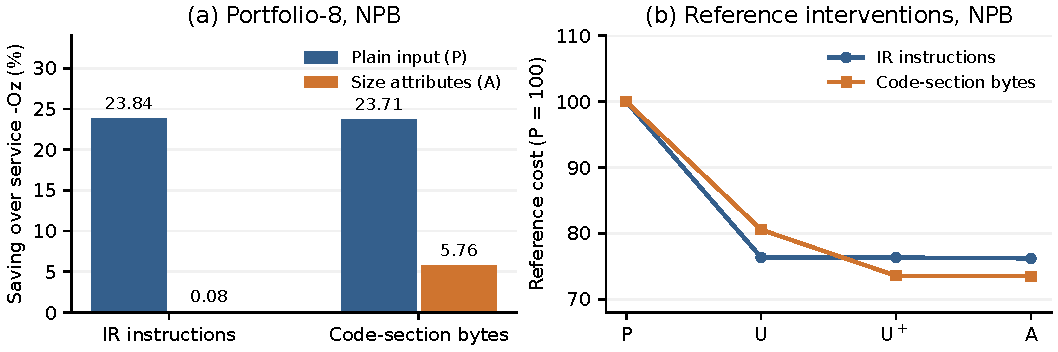
\includegraphics[width=\textwidth]{figures/baseline_audit.pdf}
\caption{The main effect and its mechanism. (a)~Portfolio-8 savings on
the \NpbCount{} NPB modules when selected by IC, before and after size
attributes are added to both sides. (b)~Reference costs under the
interventions, normalized separately to P. U$^+$ changes attributes
only before code generation. These are deterministic cohort totals,
not estimates of a population mean.}
\label{fig:main}
\end{figure*}

\section{Results}
\subsection{Baseline sensitivity is large on NPB}
Table~\ref{tab:paired} reports both preparations and both methods.
The portfolio's NPB IC gain changes from \NpbPlainIcGain\% to
\NpbAttrIcGain\%, while code-section savings change from
\NpbPlainCodeGain\% to \NpbAttrCodeGain\%.
The random control has the same qualitative behavior: its apparent
IC gain becomes a loss, while a code-section saving remains.
The effect is smaller on MiBench and absent in the BLAS IC comparison.
Thus neither the magnitude of the NPB effect nor disappearance of the
IR gain should be generalized to all suites or all size metrics.

\begin{table}[t]
\caption{Savings over the service reference (\%). Candidates are selected
by IC in every column. P/A: without/with size attributes on both sides.}
\label{tab:paired}
\centering\small
\setlength{\tabcolsep}{3.5pt}
\begin{tabular}{@{}llrrrr@{}}
\toprule
 & & \multicolumn{2}{c}{IC} & \multicolumn{2}{c}{Code bytes} \\
Suite ($n$) & Method & P & A & P & A \\
\midrule
\PairedRows
\bottomrule
\end{tabular}
\end{table}

For attributed NPB inputs, the portfolio wins/ties/loses on
\NpbIcWins/\NpbIcTies/\NpbIcLosses{} modules in IC, and
\NpbCodeWins/\NpbCodeTies/\NpbCodeLosses{} in code bytes.
The almost-zero summed IC gain therefore does not imply identical
results per module. Candidate outputs can also change when attributes
are added; the paired result is not a change of the denominator alone.

\subsection{Unrolling explains almost all reference IC inflation}
The original reference contains \PlainIc{} instructions; U has
\UnrollIc{}, and A has \AttrIc{}. Preventing unrolling removes
\UnrollIcDelta{} of the \AttrIcDelta{} instructions separating P
and A. The replica reports \UnrolledLoops{} fully unrolled loops
on \UnrolledModules{} modules under P, and none under A.
On each of these \UnrolledModules{} modules, U and A have the same
IC and the same complete IR after normalizing size attributes and loop
metadata. AU and A have identical metrics throughout the cohort.
The residual \ResidualIc{} instructions occur on \ResidualModules{}
modules with no unrolling; IR differences suggest attribute-sensitive
inlining and instruction combining, which were not separately ablated.

This evidence goes beyond attributing every difference to an
optimization flag. A targeted intervention reproduces almost the
entire reference IC change in the original service. It measures the
effect of preventing unrolling and the subsequent pipeline behavior;
it is not a universal additive partition of compiler decisions.

\subsection{Code generation accounts for a further byte effect}
For code sections, P, U, and A total \PlainCode{}, \UnrollCode{},
and \AttrCode{} bytes. U$^+$ has exactly U's IC but saves
\LateCodeDelta{} more bytes, leaving it only \LateCodeResidual{}
bytes above A. For \SameIrModules{} of the \NpbCount{} modules,
U and A have identical normalized IR and U$^+$ produces the same
object bytes as A. Removing the attributes from A before code
generation reverses this equality on those modules.

The attribution depends on the order of interventions. Adding the
attributes late to P saves \PlainLateCodeDelta{} bytes; adding them
late to U saves \LateCodeDelta{}. We therefore report these controlled
differences rather than assigning an invariant percentage of the total
byte gap to each cause. Berkeley text likewise falls from
\PlainBerkeley{} through \UnrollBerkeley{} to \AttrBerkeley{} bytes,
but it is a different quantity from executable code sections.

\subsection{A concrete function exposes the mechanism}
We extract \texttt{transfb\_nc0} unchanged from NPB module 116 using
\texttt{llvm-extract}. Its original C source is unavailable; no source
is reconstructed. The function contains a $5\times3$ loop nest.
Under P the nest expands to 15 copies of its body, leaving
\ExamplePlainIc{} IC and \ExamplePlainBytes{} function bytes.
U retains the loops at \ExampleUnrollIc{} IC and
\ExampleUnrollBytes{} bytes. A has the same IC but only
\ExampleAttrBytes{} bytes; adding attributes late to U produces that
same size. The function body and size match those in the full-module
objects, so extraction did not create this effect.

The artifact includes the input IR, transformed IR, objects and a
driver. All variants agree bit for bit on four fixed pseudorandom
input vectors and all 25 outputs per vector. This is a regression
check, not a semantic-equivalence proof. The example illustrates the
cohort-level intervention; it is not a separate independent benchmark.

\subsection{Source builds and candidate selection bound the claim}
Adding attributes does not reproduce every decision of a source build.
For \SourceCount{} CHStone programs~\cite{chstone}, the plain service,
attributed service, and direct \texttt{clang -Oz} builds contain
\SourcePlainBytes{}, \SourceAttrBytes{}, and \SourceClangBytes{}
code-section bytes, respectively. The attributed service is
\SourceAttrOverClang\% larger in aggregate, but GSM remains
\GsmOverClang\% larger. Closeness of the pooled sum is not evidence
of per-program equivalence. This source control is confined to CHStone.

A secondary audit examines \SelectorCount{} programs under A, with
eight candidates per generator: three stored GNN checkpoints and five
random realizations. Selecting the same pools directly by code bytes
yields GNN savings of \GnnCodeMin--\GnnCodeMax\% and random savings
of \RandomCodeMin--\RandomCodeMax\%. The GNN has a lower summed IC
than every random realization under IC selection, but no consistent
code-byte advantage across generator pairings under byte selection.
This is not evidence of equivalence, and the policy was not retrained
under the new preparation. The broader Berkeley-text metric gives
different conclusions: Berkeley-first GNN selection saves
\GnnBerkeleyWithoutMin--\GnnBerkeleyWithoutMax\% even without NPB,
where code-first code-section savings are close to zero or negative.
Full paired records are provided separately to keep this check
distinct from the causal NPB experiment.

\section{Scope and Practical Implications}
The strongest result is specific to LLVM~10, the original service
pipeline, the frozen candidates, and the stated cohorts. The NPB
modules are related and the cohort was inherited from the earlier
experiment. We do not estimate how often this effect occurs across
arbitrary software, and we have not audited the references of other
publications. The direct source-build control does not establish
equivalence for the NPB inputs. No end-to-end optimization time,
execution-time improvement, or linked-binary saving is claimed.

IC agreement is checked exactly, but bitcode serialization can differ
for identical IR. One unselected candidate in the secondary audit also
has two object hashes with equal measured sizes. We retain these
distinctions rather than equating cost reproduction with universal
bitwise determinism. Fixed-vector tests do not prove correctness for
all inputs. The candidate-selection ranges describe the observed
checkpoints and realizations, not confidence intervals or the outcome
of retraining.

For a size-oriented evaluation, the input attributes should be stated
alongside the pass pipeline. Reference and candidate inputs should
have matched preparation, with source-level comparisons where possible.
IR counts, code sections and broader object size should be reported as
separate objectives. A random control at the same candidate budget
helps distinguish the effect of learned generation from the effect of
search and selection. These practices define the comparison; they do
not require every size-oriented task to use one universal attribute set.

\section{Conclusion}
In the audited experiment, input preparation changes the apparent
portfolio IC advantage on NPB from \NpbPlainIcGain\% to
\NpbAttrIcGain\%. A targeted unrolling intervention explains nearly
all of the reference's IC change, while a fixed-IR control reveals a
further code-generation effect. A \NpbAttrCodeGain\% code-section
saving nevertheless survives. The result demonstrates why a gain
over an IR pipeline must be interpreted with its input attributes and
its actual size metric, rather than automatically as a gain over
source-level compilation for size.

\textbf{Artifact.} Source, per-module records, numerical checks and
the executable example are available at
\url{https://github.com/dimitrijepesic/compiler-opt}.
The figure and numerical macros are generated from recorded results;
the repository separates record verification from rerunning the compiler.

\section*{Acknowledgment}
The author thanks Prof.~Zaharije Radivojevi\'c for early discussions of
this work.

\bibliographystyle{IEEEtran}
\bibliography{main}
\end{document}
